\documentclass[UTF8]{article}
%\renewcommand\abstractname{Abstract}
%\renewcommand\contentsname{Content}
%\renewcommand{\thetable}{}
\usepackage{CTEX}
\usepackage{CJKutf8}
\usepackage{fancyhdr}
\pagestyle{fancy}
\lhead{A201800682}
\chead{第六届泰迪杯数据挖掘挑战赛}
\rhead{}
\lfoot{}
\cfoot{\small\sffamily 第\thepage页\quad共\pageref{LastPage}页}
\rfoot{}
\usepackage[russian]{babel}
\let\captionsrussian\empty
\let\daterussian\empty
\usepackage{caption}
\usepackage{subfigure}
\usepackage[explicit]{titlesec}
\usepackage{lastpage}
\usepackage{listings}
\usepackage{color}
\usepackage{hyperref}
\hypersetup{colorlinks=true,linkcolor=black}
\definecolor{dkgreen}{rgb}{0,0.6,0}
\definecolor{gray}{rgb}{0.5,0.5,0.5}
\definecolor{mauve}{rgb}{0.58,0,0.82}
\lstset{ %
  language=Octave,                % the language of the code
  basicstyle=\footnotesize,           % the size of the fonts that are used for the code
  numbers=left,                   % where to put the line-numbers
  numberstyle=\tiny\color{gray},  % the style that is used for the line-numbers
  stepnumber=2,                   % the step between two line-numbers. If it's 1, each line 
                                  % will be numbered
  numbersep=5pt,                  % how far the line-numbers are from the code
  backgroundcolor=\color{white},      % choose the background color. You must add \usepackage{color}
  showspaces=false,               % show spaces adding particular underscores
  showstringspaces=false,         % underline spaces within strings
  showtabs=false,                 % show tabs within strings adding particular underscores
  frame=single,                   % adds a frame around the code
  rulecolor=\color{black},        % if not set, the frame-color may be changed on line-breaks within not-black text (e.g. commens (green here))
  tabsize=2,                      % sets default tabsize to 2 spaces
  captionpos=b,                   % sets the caption-position to bottom
  breaklines=true,                % sets automatic line breaking
  breakatwhitespace=false,        % sets if automatic breaks should only happen at whitespace
  title=\lstname,                   % show the filename of files included with \lstinputlisting;
                                  % also try caption instead of title
  keywordstyle=\color{blue},          % keyword style
  commentstyle=\color{dkgreen},       % comment style
  stringstyle=\color{mauve},         % string literal style
  escapeinside=``,            % if you want to add LaTeX within your code
  morekeywords={*,...}               % if you want to add more keywords to the set
}
\usepackage{tabularx}  
\usepackage{graphicx}
\graphicspath{{fig/}}
\usepackage{enumerate}
\usepackage{geometry}
%\geometry{left=1cm,right=1cm,top=2cm,bottom=2cm}
\usepackage{amsmath}
 \usepackage{amssymb} 
\usepackage{multicol}
\usepackage{indentfirst}
\setlength{\parindent}{2em}
\title{\textbf{基于信噪比的非侵入式负荷检测与分解}}
\author{}
\date{}
\begin{document}
%\begin{CJK}{UTF8}{gkai}
\maketitle
%\end{CJK}
\begin{abstract}
本文主要研究的是非侵入式负荷检测与分解。在经过数据预处理后,依次考察了已知操作记录的单一态、未知操作记录的单一态、未知操作记录已知设备的复合态和未知操作记录未知设备的复合态数据,建立了合理的基于信噪比的特征识别模型,成功识别了用电设备并得出噪声的分布函数,并与识别结果的噪声值比较判断正确的可能性。\\
\indent 在数据预处理阶段,我们依次进行了对空缺数据的插值、对粗大误差的校正、对零点误差的校正和对噪声的平滑滤波。\\
\indent 针对问题一,我们将附件一经过预处理的数据当作不含噪声的真实值。利用特征识别的方法获得暂态特征和稳态特征,并用一个函数量化这些特征。\\
\indent 针对问题二、三,我们用同样的方法得到未知设备的负载印记的特征函数。通过计算信噪比判断未知设备的暂态特征函数最可能是从问题一已知的哪一个暂态特征函数,进而得到未知设备的代号和操作记录。\\
\indent 针对问题四,我们如果发现有未知设备的负载印记的特征函数跟所有已知的特征函数匹配的信噪比值远远小于问题二、三获得的信噪比数据,则怀疑是否出现YD0,进行假设检验。如果无法通过检验,则认为出现YD0。\\
\indent 对叠加态的分解结果利用0-1线性规划模型计算噪声,利用噪声分布的概率分布函数,计算得到出现小于该噪声的概率为87.3\%。\\
\end{abstract}
\textbf{关键词}:非侵入式负荷检测与分解;特征识别;信噪比;0-1线性规划;假设检验。

\newpage
\thispagestyle{empty}
\begin{center}
\Large
\textbf{}\\
\normalsize
\textbf{Summary}
\end{center}
\small

This paper is mainly about the research of non intrusive load detection and decomposition. After data preprocessing, the single state of the known operating records, the single state of unknown operation records, the complex state of unknown operating records and the complex state data of unknown operating records are investigated in turn, and a reasonable feature recognition model based on the signal to noise ratio is established, and the power equipment is successfully identified and obtained. The distribution function of noise is obtained, and the probability of correctness is judged by comparing with the noise value of the recognition result.\\
\indent In the data preprocessing phase, we interpolate the vacancy data, correct the rough error, correct the zero point error and smooth the noise.\\
\indent For problem one, we use Annex I preprocessed data as the real value without noise. We use feature recognition to get transient features and steady-state features, and quantify these characteristics with a function.\\
\indent For problem two or three, we use the same method to get the characteristic function of the load imprint of the unknown device. By calculating the signal to noise ratio, the transient characteristic function of the unknown equipment is most likely to be a known transient characteristic function from the problem, and then the code and operation record of the unknown equipment are obtained.\\
\indent For problem four, if we find that the signal-to-noise ratio of the characteristic function of the unknown device's load imprint and all the known feature functions is far smaller than the signal to noise ratio data obtained by problem two or three, it is doubtful whether or not to appear YD0 for hypothesis testing. If the test cannot be passed, YD0 is considered to appear.\\
\indent The result of the decomposition of the superposition state is calculated by the 0-1 linear programming model. The probability distribution function of noise distribution is calculated to be 87.3\% less than the noise. \\
\textbf{Keywords}:Non Intrusive Load Detection and Decomposition; Feature Recognition; Signal-to-noise Ratio; 0-1 Linear Programming; Hypothesis Testing.
\normalsize

\newpage
\thispagestyle{empty}
\tableofcontents
\newpage
\setcounter{page}{1}
\section{引言}
随着经济社会的发展,居民用户家中的用电器数量也不断增加。为了更好地评价建筑节能水平、促进节能环保、保证电网安全运行,通过异常的用电数据对设备老化和故障进行预警,对电力进行分项计量趋于必要。相比于传统的给所有用电设备加装电力计量装置和通信装置的侵入式电力负荷监测带来的成本高、施工复杂、干扰用户正常生活等不便,非侵入式电力负荷监测与分解可以很好的解决这些问题。

\section{问题重述}
\begin{enumerate}[1]
\item 根据附件1提供的单一态数据,分析并给出各用电设备的运行特征,并估计各用电设备的实时用电量(文件名为energy1.xlsx,表名分别为YD1、YD2、……、YD11,结果格式参见表6,其中各变量的含义见表7)。
\item 根据附件2中的单一态数据,设计自动识别单一设备的数学模型和计算方法,并估计这一用电设备的实时用电量(文件名为energy2.xlsx,表名分别为设备1、设备2、设备3,结果格式参见表6)。
\item 根据附件3提供的用电设备实测数据,设计方法确定各用电设备的状态、操作及操作时间(文件名为operation3.xlsx,表名分别为设备组1、设备组2、设备组3,结果格式参见表5),并估计每个用电设备的实时用电量(文件名为energy3.xlsx,表名分别为设备组1、设备组2、设备组3,结果格式参见表6)。
\item 利用问题3设计的方法,根据附件4提供的用电设备实测数据,识别出各用电设备及其状态、操作及操作时间(文件名为operation4.xlsx,表名分别为设备组1、设备组2、设备组3,结果格式参见表5),并估计每个用电设备的实时用电量(文件名为energy4.xlsx,表名分别为设备组1、设备组2、设备组3,结果格式参见表6),无法识别的用电设备标记为YD0。
\end{enumerate}

\section{假设与标记}
\subsection{假设}
\begin{enumerate}[1]
\item 2个用电设备依次发生状态改变的时间间隔充分大以便于我们可以正确检测出它们。
\item 噪声的频率分布服从正态分布。
\end{enumerate}

\subsection{标记}
\begin{table}[htbp]
\centering
\caption{变量的定义}
\begin{tabular}{|c|l|}
\hline
变量&定义\\
\hline
\(u\)&电压\\
\hline
\(v\)&电压相扰动\\
\hline
\(i\)&电流\\
\hline
\(p\)&有功功率\\
\hline
\(q\)&无功功率\\
\hline
\(t\)&时间\\
\hline
\(\omega\)&频率\\
\hline
\(e\)&噪声\\
\hline
SNR&信噪比\\
\hline
\end{tabular}
\end{table}

\section{问题分析}
\begin{enumerate}[1]
\item 我们选取的运行特征包括电器在暂态和稳态的电压相扰动、电流在时域和频域的图像。先对数据进行预处理,然后提取相应特征。对于实时用电量,将有功功率单位换算成千瓦时。
\item 对于未知设备的单一态用同样的方式得到运行特征,先假设该设备为某一已知用电设备的某一特征,获得其信噪比。假如假设成立,该信噪比应该随噪声趋于0而趋于无穷大,所以将信噪比最大的假设视为真。
\item 对于未知设备的叠加态,获得其功率的运行特征,先采用信噪比的判别方法,判断用电设备的种类;\\
再利用0-1线性规划模型检验该叠加态的分解是否合理。
\item 对于可能存在未知设备YD0的情况,使用假设检验的方法判别是否出现。用误差的历史数据拟合出误差的分布函数。若在不存在YD0的情况下出现该误差的概率小于\(p\),判定假设为假,相信YD0已经出现。
\end{enumerate}

\section{用于特征识别的信噪比比较模型}
\subsection{模型的建立}
\paragraph{数据预处理}
\subparagraph{插值}
\indent 对于实时用电量,YD1、YD2的数据在时间上存在空缺。对于缺少的数据,根据稳态的特征予以插值,例如风扇一档的设备数据几乎不变,空调睡眠状态的设备数据呈周期性变化。
\begin{figure}[htbp]
\centering
\begin{minipage}[htbp]{7cm}
\centering
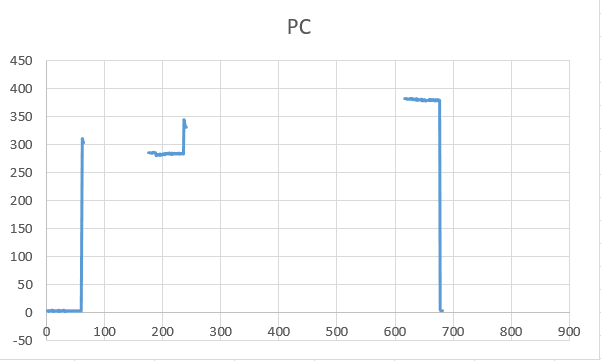
\includegraphics[width=6cm]{i1.png}
\caption*{子图 1:插值前}
\end{minipage}
\begin{minipage}[htbp]{7cm}
\centering
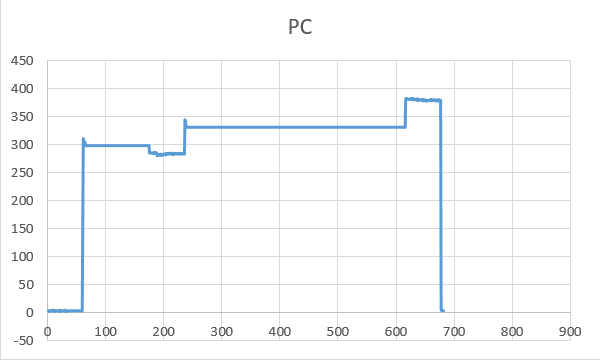
\includegraphics[width=6cm]{i2.png}
\caption*{子图 2:插值后}
\end{minipage}
\caption{对空缺值的处理}
\end{figure}

\subparagraph{处理粗大误差}
\indent 发现电压电流的周波数据主要集中在0和1666650这2个相差较远的值范围,不符合正常周波应接近正弦波的规律。考虑到仪器读取数据可能存在读取错误的问题,对集中在1666650的数据进行平移,发现可以转化为接近正弦波的图像,验证了我们的猜想。
\begin{figure}[htbp]
\centering
\begin{minipage}[htbp]{7cm}
\centering
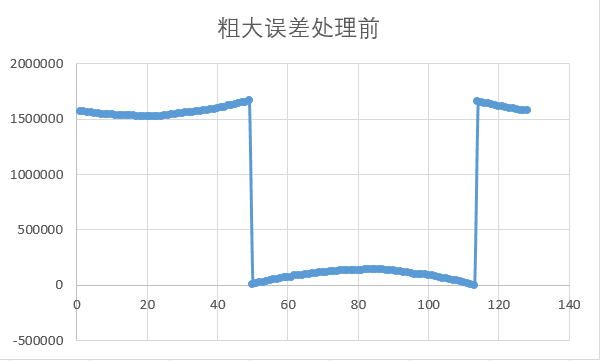
\includegraphics[width=6cm]{g1.png}
\caption*{子图 1:粗大误差处理前}
\end{minipage}
\begin{minipage}[htbp]{7cm}
\centering
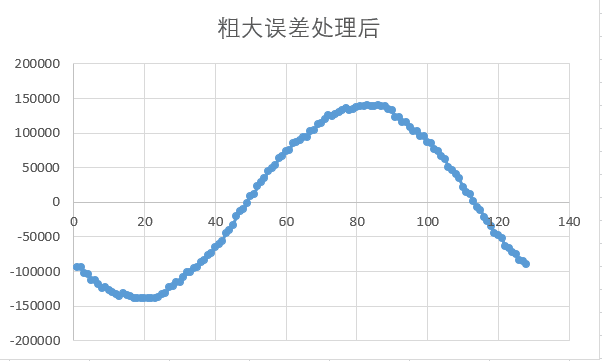
\includegraphics[width=6cm]{g2.png}
\caption*{子图 2:粗大误差处理后}
\end{minipage}
\caption{处理粗大误差}
\end{figure}

\subparagraph{处理零点误差}
\indent 在设备处于关闭状态时电流和功率仍有数值,考虑到零点漂移,统一将数据减去零点误差,并将关闭状态的设备数据按0计算。
\begin{figure}[htbp]
\centering
\begin{minipage}[htbp]{7cm}
\centering
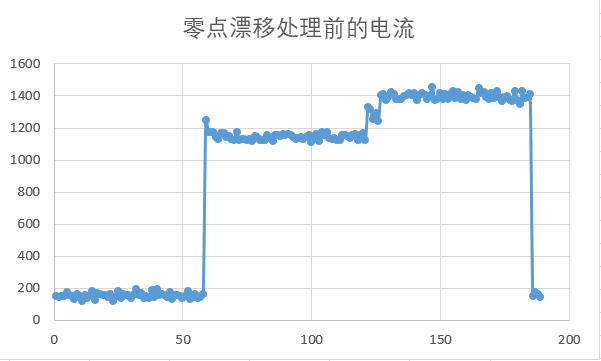
\includegraphics[width=6cm]{z1.png}
\caption*{子图 1:零点误差处理前}
\end{minipage}
\begin{minipage}[htbp]{7cm}
\centering
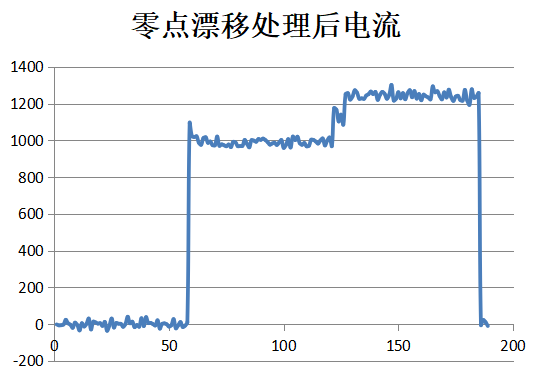
\includegraphics[width=6cm]{z2.png}
\caption*{子图 2:零点误差处理后}
\end{minipage}
\caption{处理零点误差}
\end{figure}

\subparagraph{滤波}
\indent 注意到数据有大量锯齿状的波动,而正常情况下这些物理量应该是光滑的。于是对数据进行滤波处理。
\begin{figure}[htbp]
\centering
\begin{minipage}[htbp]{7cm}
\centering
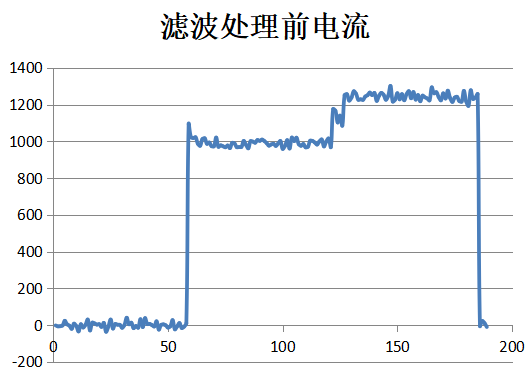
\includegraphics[width=6cm]{f1.png}
\caption*{子图 1:平滑滤波前}
\end{minipage}
\begin{minipage}[htbp]{7cm}
\centering
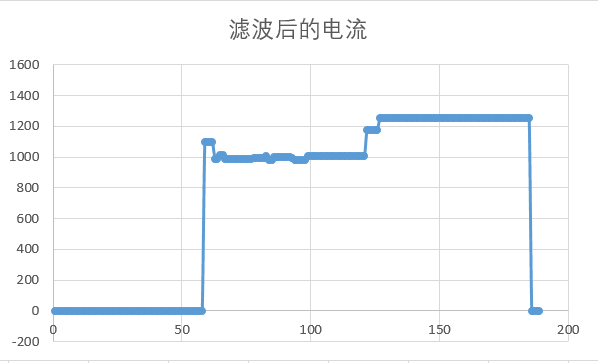
\includegraphics[width=6cm]{f2.png}
\caption*{子图 2:平滑滤波后}
\end{minipage}
\caption{平滑滤波}
\end{figure}

\subparagraph{处理频域}
\indent 频域的分布与电器的阻抗有关,对于不同时刻的电器,其频谱相似度较高,可以作为负载印记。
\begin{figure}[htbp]
\small
\centering
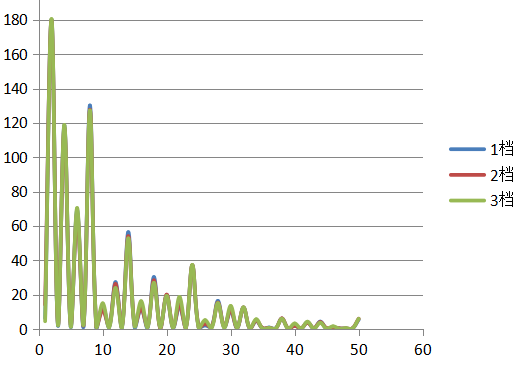
\includegraphics[width=8cm]{h.png}
\caption{频域特征}
\end{figure}

\paragraph{特征提取}
\indent 经过数据预处理后,我们得到了每种用电设备的相对正确的数据。因为空缺的数据都是稳态,所以提取特征时使用了未插值但经过了零点校正和平滑滤波的周波基数据。进行下面分已知操作记录和未知操作记录两种情况分别讨论。
\subparagraph{已知操作记录}
\indent 我们从每次操作处理后开始计时,直到数据停止波动。我们将数据在一段时间\(\tau\)内极差小于\(\varepsilon\)视为停止波动。具体的\(\tau\)和\(\varepsilon\)值经过尝试后取值。我们将某一暂态特征的采样数据按时间顺序从0开始排列,并称数据关于时间的函数为该暂态特征的特征函数。但实际上由于采样频率是每秒1次的原因,这只是一个有穷数列,所以也可以称之为暂态特征的特征向量。\\
\indent 对于稳态特征,因为理想情况下的稳态特征向量都具有周期性,所以可按数据是否随时间变化细分为常数性稳态和非常数性稳态。截取其一个最小正周期(非常函数)或一个采样周期(常函数)作为稳态特征向量的维度。

\subparagraph{未知操作记录}
\begin{figure}[htbp]
\small
\centering
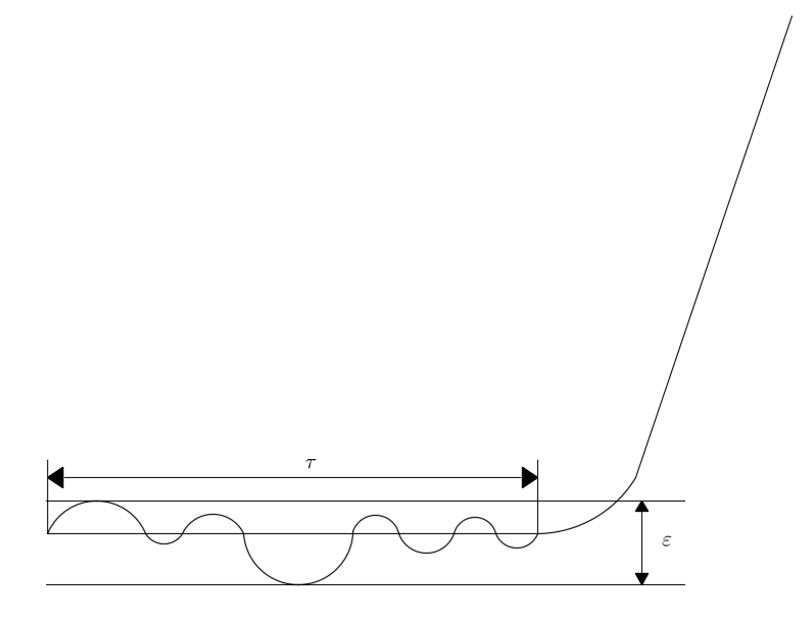
\includegraphics[width=8cm]{idea.png}
\caption{暂态判别示意图}
\end{figure}
\begin{enumerate}[1]
\item 对于未知操作记录的数据,在最开始,电器都处于关闭状态(稳态),之后才启动(暂态)。不妨假设噪声最大为\(\varepsilon\),一旦一段时间\(\tau\)内数据极差小于\(\varepsilon\),我们就认为存在某一设备进入了暂态。
\item 同样,一旦一段时间\(\tau\)内设备的波动没有大于\(\varepsilon\),我们就认为该设备回到了稳态。我们记录下每一个暂态开始的时间。然后开始寻找下一个暂态开始的时刻。
\item 重复以上过程,我们获得了所有的暂态特征。
\end{enumerate}

每两个相邻的暂态特征之间必定是稳态特征。所以仿照已知操作记录的情况进行特征提取。\\
\indent 对所有相邻的暂态特征进行处理,我们获得了所有的稳态特征。对于单一态的数据,稳态特征可以直接用于特征识别;对于叠加态还要进行分解才能获得每个用电设备的稳态特征。

\paragraph{特征识别}
\subparagraph{不存在YD0}
\indent 对于每一个负载印记,我们计算假设它为某一用电设备的某一特征时的信噪比,将信噪比最大的假设视为真。\\
\indent 例如,对于未知的暂态特征向量\(g(t)\),我们假设它其实是某一用电设备的暂态特征\(f(t)\)。我们计算噪声为
\[N=\sqrt{\int\limits_0^T\big(f(t)-g(t)\big)^2\textrm{d}t}\]
\indent \(f(t)\)的信号强度为
\[S=\sqrt{\int\limits_0^T\big(f(t)\big)^2\textrm{d}t}\]
\indent 则信噪比为
\[S/N=\sqrt{\frac{\int\limits_0^T\big(f(t)-g(t)\big)^2\textrm{d}t}{\int\limits_0^T\big(f(t)\big)^2\textrm{d}t}}\]
\indent 但信噪比数量级太大,不利于比较。我们通常会取对数,用分贝作为单位:
\[\textrm{SNR}=20\textrm{lg}\sqrt{\frac{\int\limits_0^T\big(f(t)-g(t)\big)^2\textrm{d}t}{\int\limits_0^T\big(f(t)\big)^2\textrm{d}t}}\]
\indent 对于每一个用电设备的每一特征\(f_i(t)\),计算得到每一个SNR\(_i\),我们认为使得SNR\(_i\)取最大值的\(f_i(t)\)就是暂态特征\(g(t)\)。

\subparagraph{可能存在YD0}
\indent 在问题四中,如果某一个特征跟所有已知用电设备假设的信噪比都低(用问题二获得的历史数据判断是否在同一个数量级),那么利用假设检验的方法判断究竟是噪声还是用电设备YD0。\\
\indent 我们假设问题一的基数据在平滑滤波前含有噪声而滤波后不含噪声,通过前者减后者,得到噪声的时间分布。计算所有噪声出现的频率。根据假设噪声服从正态分布。所以利用正态分布函数用噪声的频率函数拟合概率密度函数。
\begin{figure}[htbp]
\small
\centering
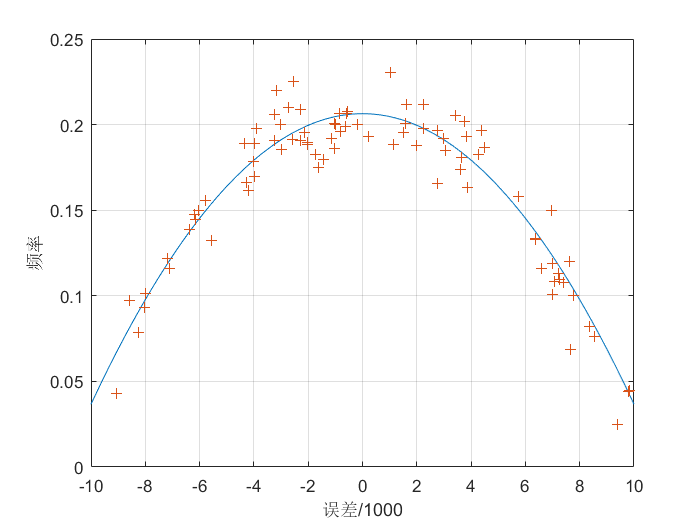
\includegraphics[width=8cm]{N.png}
\caption{噪声分布}
\end{figure}\\
\indent 假设\(H_0\):该现象是噪声导致的。\\
\indent 假设\(H_1\):该现象不是由噪声导致的。即出现了未知的用电设备YD0。\\
\indent 如果该噪声的分布函数值大于\(1-p\),认为这是小概率事件,拒绝假设\(H_0\),相信假设\(H_1\)。\\

\subsection{模型的求解}
\begin{enumerate}[1]
\item 问题一中用电设备的实时用电量如附件energy1.xlsx所示。
\item 问题二中设备一为YD10,即电吹风。设备二为YD9,即空调。实时用电量见附件energy2.xlsx。
\item 问题三中设备的操作记录和实时用电量分别见附件operation3.xlsx和energy3.xlsx。
\item 问题三中设备的操作记录和实时用电量分别见附件operation4.xlsx和energy4.xlsx。
\end{enumerate}

\subsection{模型的检验}
\subsubsection{灵敏度检验}
\indent 本题主要利用了\(p\)、\(\varepsilon\)和\(\tau\)这3个参数。对这3个参数进行修改后发现,将\(p\)从0.05改成0.1后判断结果仍然一致。而模型对\(\varepsilon\)和\(\tau\)的依赖程度较大,主要原因是\(\varepsilon\)和\(\tau\)这2个参数来源于问题1的历史数据,而该数据中噪声普遍集中在\(\varepsilon\)附近,一旦减少\(\varepsilon\),就有可能将噪声和真正的暂态分辨错误。对\(\tau\)同理。

\subsubsection{基于0-1线性规划模型的误差检验}
\indent 问题三、四提供了叠加态特征\(p(t)\)。有
\[p(t)=\sum\limits_{i=1}^{n}\sum\limits_{j=1}^{m(i)}X_{ij}(t)p_{ij}(t)+e(t)\]
\indent 其中,第\(i\)种设备的第\(j\)个稳态特征为\(p_{ij}(t)\)。假设一共有\(n\)种用电设备,第\(i\)种用电设备一共有\(m(i)\)个稳态特征。\(e(t)\)为噪声。\(X_{ij}(t)\)为示性函数,当且仅当在时刻\(t\)第\(i\)种设备工作于第\(j\)个稳态特征时,\(X_{ij}(t)=1\),否则\(X_{ij}(t)=0\)。\\
\indent 于是,可能性最大的\(X_{ij}(t)\)必然能使噪声\(e(t)\)最小。
\[\textrm{min }e(t)\]
\[\textrm{s.t.}\left\{
\begin{array}{l}
p(t)=\sum\limits_{i=1}^{n}\sum\limits_{j=1}^{m(i)}X_{ij}(t)p_{ij}(t)+e(t)\\
\sum\limits_{j=1}^{m(i)}X_{ij}(t)\leqslant1\\
X_{ij}(t)\in\{0,1\}
\end{array}\right. \]
\indent 事实上无须依靠求解该问题得到操作记录。暂态特征和稳态特征是相互联系的。出现暂态特征必伴随着稳态特征的变化。我们可以通过已经求出的操作记录得到所有叠加态的稳态特征的分解结果,将每一叠加态的分解结果代入该模型计算每一叠加态的噪声\(\varepsilon\),根据噪声的概率密度函数积分得到噪声出现的概率分布函数,再查出该噪声出现的概率,判断我们通过信噪比建立的特征识别模型是否可信。所有叠加态的平均噪声为\(0.37\times10^4\),出现的概率为87.3\%。可信度较高。

\section{模型的评价与改进}
\subsection{优点}
\begin{enumerate}[1]
\item 很好地解决了题目提出的问题,模型简单而有效。
\item 利用信噪比进行特征匹配,想法新颖而效果显著。对YD0的检验也不失价值。
\end{enumerate}

\subsection{缺点}
\begin{enumerate}[1]
\item 特征匹配时容易发生大功率电器掩盖小功率设备的情况。
\item 对非常数性稳态的识别的情况较差。
\item 没有充分利用所有数据。
\end{enumerate}

\subsection{推广}
\begin{enumerate}[1]
\item 除了电器的特征识别,对工厂里众多机器使用燃料等的情况也可模仿该题进行建模。
\end{enumerate}

\subsection{展望}
\begin{enumerate}[1]
\item 注意到谐波数据只和电器工作原理有关,可以考虑未来将所有相似工作原理的电器进行分类,以便更好地使用这一模型。
\end{enumerate}

\newpage
\begin{thebibliography}{}
\bibitem{1}\url{https://wenku.baidu.com/view/db5d862924c52cc58bd63186bceb19e8b8f6ec31.html}
\bibitem{2}黎鹏. 非侵入式电力负荷分解与监测[D].天津大学,2009.
\end{thebibliography}
\addcontentsline{toc}{section}{参考文献}
\addcontentsline{toc}{section}{附录}

\begin{appendix}
\section{代码}
\begin{lstlisting}[title=数据预处理.m, frame=shadowbox]
a=xlsread('   ',2 ,':');
if(a<1000000)
a=a;
else
a=a-1666665;
b=xlswrite('   ',a,4,' : ');
\end{lstlisting}
\begin{lstlisting}[title=数据处理(周波).m, frame=shadowbox]
a=xlsread('   ',2 ,':');
b=max(a);
c=min(a);
d=(b-c)/2.83;
y=size(A,2);
plot(y,d);
\end{lstlisting}
\begin{lstlisting}[title=数据处理(谐波).m, frame=shadowbox]
a1=xlsread('   ',2 ,':');
b1=average(a);
B=[b1,b2,....b50];
x=1:50;
plot(x,B);
\end{lstlisting}
\begin{lstlisting}[title=信噪比模型.m, frame=shadowbox]
a=xlsread('   ',2 ,':');
b=xlsread('   ',2 ,':');
c=a-b
N=sqrt(sum((a-b).^2(:)));
S=sqrt(sum(a.^2(:))-sum(b.^2(:)));
R=S/N 
SNR=20*log10(R);
\end{lstlisting}
\begin{lstlisting}[title=特征识别0-1线性规划.m, frame=shadowbox]
x=xlsread('   ',2 ,':')
x=[   ;   ;   ;   ];
for(a=0:1)
 for(b=0:1)
  for(c=0:1)
   for(d=0:1)
p=[ a;b ;c ;d ];
pp=p'
q=xlsread('   ',2 ,':');
e=q-x*pp;
emin=min(e);

d=xlsread('C:\Users\qxh\Desktop\taidibei\A\`{\color{mauve}{附件1}}`\YD2',5,'EB2:EB785');
e=xlsread('C:\Users\qxh\Desktop\taidibei\A\`{\color{mauve}{附件1}}`\YD3',5,'EB2:EB136');
f=xlsread('C:\Users\qxh\Desktop\taidibei\A\`{\color{mauve}{附件1}}`\YD4',5,'EC2:EC938');
g=xlsread('C:\Users\qxh\Desktop\taidibei\A\`{\color{mauve}{附件1}}`\YD5',5,'EC2:EC125');
h=xlsread('C:\Users\qxh\Desktop\taidibei\A\`{\color{mauve}{附件1}}`\YD6',5,'EC2:EC122');
i=xlsread('C:\Users\qxh\Desktop\taidibei\A\`{\color{mauve}{附件1}}`\YD7',5,'EC2:EC420');
j=xlsread('C:\Users\qxh\Desktop\taidibei\A\`{\color{mauve}{附件1}}`\YD8',5,'EC2:EC689');
k=xlsread('C:\Users\qxh\Desktop\taidibei\A\`{\color{mauve}{附件1}}`\YD9',5,'ED2:ED212');
l=xlsread('C:\Users\qxh\Desktop\taidibei\A\`{\color{mauve}{附件1}}`\YD10',5,'EC2:EC503');
m=xlsread('C:\Users\qxh\Desktop\taidibei\A\`{\color{mauve}{附件1}}`\YD11',5,'EC2:EC127');
a=xlsread('C:\Users\qxh\Desktop\taidibei\A\`{\color{mauve}{附件1}}`\YD1',4,'F3:BC3');
b=xlsread('C:\Users\qxh\Desktop\taidibei\A\`{\color{mauve}{附件1}}`\YD1',4,'F4:BC4');
c=xlsread('C:\Users\qxh\Desktop\taidibei\A\`{\color{mauve}{附件1}}`\YD1',4,'F5:BC5'); 
a=xlsread('C:\Users\qxh\Desktop\taidibei\A\`{\color{mauve}{附件1}}`\YD1',4,'F3:BC3');
b=xlsread('C:\Users\qxh\Desktop\taidibei\A\`{\color{mauve}{附件1}}`\YD1',4,'F4:BC4');
c=xlsread('C:\Users\qxh\Desktop\taidibei\A\`{\color{mauve}{附件1}}`\YD1',4,'F5:BC5'); 
aa=smooth(a)
bb=smooth(b)
cc=smooth(c)
dd=smooth(d)
ee=smooth(e)
ff=smooth(f)
gg=smooth(g)
hh=smooth(h)
ii=smooth(i)
jj=smooth(j)
kk=smooth(k)
ll=smooth(l)
mm=smooth(m)
\end{lstlisting}

\section{数据}
\begin{table}[htbp]
\centering
\caption{数据}
\begin{tabular}{|c|l|c|}
\hline
符号&意义&数值\\
\hline
\(p\)&假设检验的概率值&0.05\\
\hline
\(\varepsilon\)&误差最大值&\(1\times10^4\)\\
\hline
\(\tau\)&误差最大持续时间&68s\\
\hline
\end{tabular}
\end{table}
\end{appendix}
\end{document}
